\documentclass[aspectratio=169, 10pt]{beamer}

% --- Packages ---
\usepackage[utf8]{inputenc}
\usepackage{graphicx}
\usepackage{booktabs}
\usepackage{tikz}
\usetikzlibrary{shapes.geometric, arrows, positioning, calc, shapes.multipart}
\usepackage{multicol}
\usepackage{pifont}

% --- Theme Setup ---
\usetheme{Madrid}
\usecolortheme{beaver}
\setbeamertemplate{navigation symbols}{}

% --- Title Information ---
\title[SecureGuard]{SecureGuard: Risk-Based Adaptive Security for MPIN Reset}
\subtitle{Challenge 6: Risk-Based Security for MPIN Reset}
\date{\today}

\begin{document}

% --- Slide 1: Title ---
\begin{frame}
    \titlepage
\end{frame}

\author[Suraj, Sagar, Aayam]{Team Members: Suraj Thapa, Shiva Sagar Yadav, Aayam Neupane}
\institute[Hackathon]{Esewa x WWF Hackathon 2026}

% --- Slide 2: Team Member Details ---
\begin{frame}{Team Member Details}
    \begin{table}
        \centering
        \footnotesize
        \begin{tabular}{|l|l|l|l|l|}
            \hline
            \textbf{Full Name} & \textbf{Email} & \textbf{Role} & \textbf{District} & \textbf{Gender} \\ \hline
            Suraj Thapa         & surajth64@gmail.com        & Lead Dev / UI & Kathmandu        & Male             \\ \hline
            Shiva Sagar Yadav   & kimdine999@gmail.com      & Backend Eng.  & Kathmandu        & Male             \\ \hline
            Aayam Neupane       & aayam.neupane1@gmail.com  & Risk Logic    & Kathmandu        & Male             \\ \hline
        \end{tabular}
    \end{table}
\end{frame}

% --- Slide 3: Problem Understanding ---
\begin{frame}{Problem Understanding}
    \begin{columns}
        \column{0.5\textwidth}
        \textbf{The Challenge:}
        \begin{itemize}
            \item MPIN reset is a critical vulnerability.
            \item Fraudsters exploit OTPs via social engineering and scripts.
        \end{itemize}

        \vspace{0.5cm}
        \textbf{Why It Matters:}
        \begin{itemize}
            \item Current systems lack \textbf{context}.
            \item Users on suspicious calls or compromised devices are treated identically to safe users.
        \end{itemize}

        \column{0.5\textwidth}
        \begin{alertblock}{Current Gap}
            No behavior-based risk scoring occurs \textbf{before} the OTP is displayed.
        \end{alertblock}
    \end{columns}
\end{frame}

% --- Slide 4: Proposed Solution ---
\begin{frame}{Proposed Solution: SecureGuard}
    \textbf{Core Concept:} Real-time risk evaluation middleware.

    \vspace{0.5cm}

    \begin{itemize}
        \item \textbf{Risk Scoring Engine:} Calculates Low, Mid, or High risk scores in milliseconds based on user context.
        \item \textbf{Adaptive UI:} Instead of a static OTP screen, the interface changes dynamically:
    \end{itemize}

    \vspace{0.3cm}

    \begin{enumerate}
        \item \textbf{Stealth Mode:} Zero friction for safe users.
        \item \textbf{Caution Mode:} Yellow warnings to build awareness.
        \item \textbf{Intervention Mode:} Full friction (timers/checks) to stop fraud.
    \end{enumerate}
\end{frame}

% --- Slide 5: Key Features ---
\begin{frame}{Key Features}
    \begin{columns}[t]
        \column{0.33\textwidth}
        \textbf{1. Signal Detection}
        \begin{itemize}
            \item \small High Value / New Payee flags.
            \item \small Unusual time detection.
            \item \small Active call status check.
            \item \small Device integrity scan.
        \end{itemize}

        \column{0.33\textwidth}
        \textbf{2. Risk Calculation}
        \begin{itemize}
            \item \small Runs real-time (before OTP).
            \item \small Outputs Low / Mid / High score.
        \end{itemize}

        \column{0.33\textwidth}
        \textbf{3. Adaptive Response}
        \begin{itemize}
            \item \small Dynamic Warning Messages.
            \item \scriptsize (e.g., "Don't share OTP")
            \item \small Interactive friction (Timers).
        \end{itemize}
    \end{columns}
\end{frame}

% --- Slide 6: User Journey ---
\begin{frame}{User Journey / Flow}
    \centering
    \scalebox{0.5}{%
        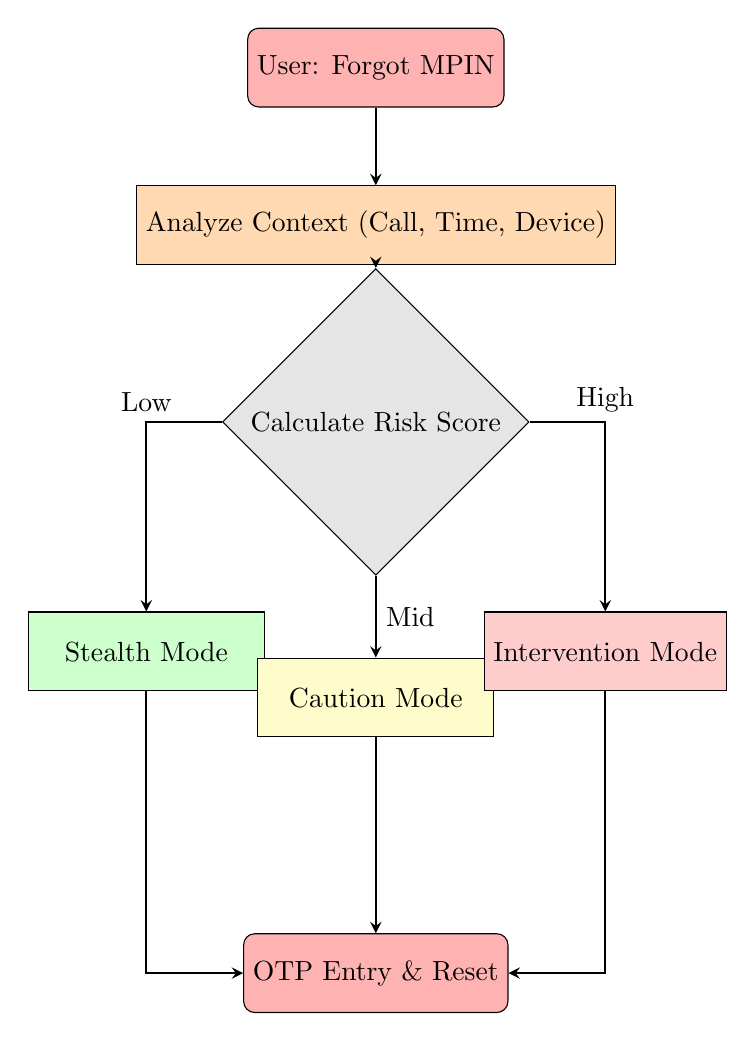
\begin{tikzpicture}[node distance=2cm]
            \tikzstyle{start} = [rectangle, rounded corners, minimum width=2.5cm, minimum height=1cm,text centered, draw=black, fill=red!30]
            \tikzstyle{process} = [rectangle, minimum width=3cm, minimum height=1cm, text centered, draw=black, fill=orange!30]
            \tikzstyle{decision} = [diamond, minimum width=3cm, minimum height=1cm, text centered, draw=black, fill=gray!20]
            \tikzstyle{arrow} = [thick,->,>=stealth]

            \node (start) [start] {User: Forgot MPIN};
            \node (context) [process, below of=start] {Analyze Context (Call, Time, Device)};
            \node (risk) [decision, below of=context, yshift=-0.5cm] {Calculate Risk Score};

            \node (low) [process, below left of=risk, xshift=-1.5cm, yshift=-1.5cm, fill=green!20] {Stealth Mode};
            \node (mid) [process, below of=risk, yshift=-1.5cm, fill=yellow!20] {Caution Mode};
            \node (high) [process, below right of=risk, xshift=1.5cm, yshift=-1.5cm, fill=red!20] {Intervention Mode};

            \node (end) [start, below of=mid, yshift=-1.5cm] {OTP Entry \& Reset};

            \draw [arrow] (start) -- (context);
            \draw [arrow] (context) -- (risk);
            \draw [arrow] (risk) -| node[anchor=south] {Low} (low);
            \draw [arrow] (risk) -- node[anchor=west] {Mid} (mid);
            \draw [arrow] (risk) -| node[anchor=south] {High} (high);
            \draw [arrow] (low) |- (end);
            \draw [arrow] (mid) -- (end);
            \draw [arrow] (high) |- (end);
        \end{tikzpicture}
    }
\end{frame}

% --- Slide 7: Architecture (Fixed Circle) ---
\begin{frame}{System Architecture}
    \centering
    \scalebox{0.55}{%
        \begin{tikzpicture}[node distance=1.5cm]
            \tikzstyle{block} = [rectangle, draw, fill=blue!10, text width=5em, text centered, rounded corners, minimum height=3em]
            \tikzstyle{server} = [rectangle, draw, fill=green!10, text width=8em, text centered, minimum height=4em]

            % FIX: Made the database cylinder much smaller and flatter
            \tikzstyle{db} = [cylinder, shape border rotate=90, draw, fill=gray!20,
            aspect=0.25, % This makes it flatter
            minimum height=1.5cm, minimum width=1.2cm,
            shape border uses custom fill,
            draw=black, top color=white, bottom color=gray!50,
            text centered, font=\footnotesize]

            \tikzstyle{line} = [draw, -latex', thick]

            \node (client) [block, fill=orange!20] {Client App (React/Mobile)};
            \node (api) [server, right=of client, xshift=2cm] {Backend API (Node.js)};
            \node (risk) [server, above=of api] {Risk Engine (Python/Logic)};
            \node (db) [db, below=of api] {Database (MongoDB)};

            \path [line] (client) -- node[above] {Request + Context} (api);
            \path [line] (api) -- node[left] {Ask Score} (risk);
            \path [line] (risk) -- node[right] {Risk Level} (api);
            \path [line] (api) -- node[right] {Logs} (db);
            \path [line] (db) -- node[left] {History} (api);
            \path [line] (api) -- node[below] {Dynamic UI Response} (client);
        \end{tikzpicture}
    }
\end{frame}

% --- Slide 8: Tech Stack & Scope ---
\begin{frame}{Technology Stack \& Scope}
    \begin{columns}
        \column{0.5\textwidth}
        \textbf{Tech Stack}
        \begin{itemize}
            \item \textbf{Frontend:} React.js / Flutter
            \item \textbf{Backend:} Node.js (Express)
            \item \textbf{Database:} MongoDB
            \item \textbf{Logic:} Python (Simulation)
        \end{itemize}

        \column{0.5\textwidth}
        \textbf{Scope}
        \begin{itemize}
            \item \textbf{In Scope:} Risk eval, Active call detection, Dynamic UI.
            \item \textbf{Out of Scope:} Biometrics, Full core banking logic.
        \end{itemize}
    \end{columns}
\end{frame}

% --- Slide 9: Secure OTP Interface ---
\begin{frame}{UI/UX Prototypes: Secure OTP Interface}
    \centering
    \textbf{Secure OTP Interface}\\
    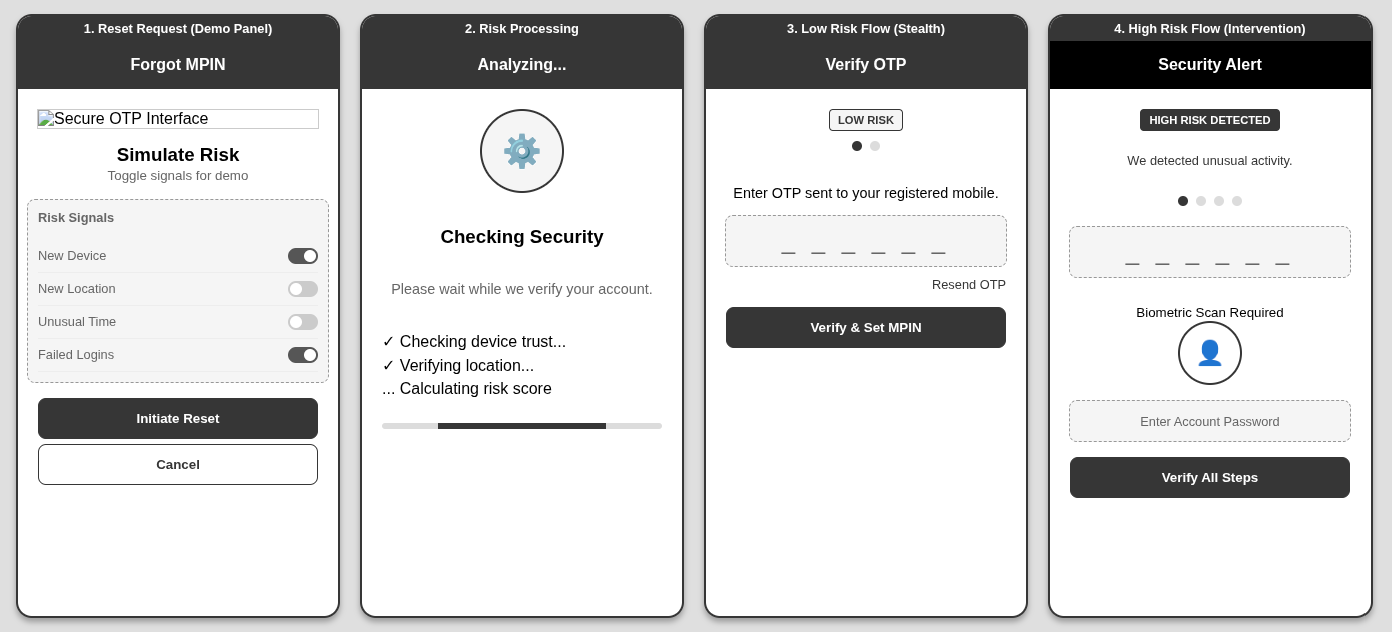
\includegraphics[height=0.7\textheight]{1.png}

    \begin{center}
        \small \textit{Clean OTP display with prominent security warning.}
    \end{center}
\end{frame}

% --- Slide 11: Impact & Conclusion ---
\begin{frame}{Expected Impact \& Conclusion}
    \textbf{Impact:}
    \begin{itemize}
        \item Stops fraud scripts by forcing user attention (Intervention).
        \item Protects against Vishing (Call detection).
        \item Zero friction for 90\% of legitimate users (Stealth mode).
    \end{itemize}

    \vspace{1cm}
    \centering
    \Large \textbf{Thank You!}\\
    \small Questions? \hspace{1cm} 
    Github Link: git@github.com:sagarEmn/esewa-hackathon-dynamic-otp-ui.git
\end{frame}

\end{document}